Presented in the proposal the reach of the experiment rely on GEANT4 and EGS5 simulations. These are well tested codes, never the less we find it is important to back-up results of simulations with experimental measurements, especially at small scattering angles where results from these simulation codes were markedly different. These simulation codes have shown that the occupancy problems in the tracker and in the ECal occur only at the very smallest angles, and are due to multiply Coulomb scattered beam electrons. To the extent that we can demonstrate that we have accurately modeled both the scattering and the response of the detector to high energy electrons which hit in and around the detector elemnts, we demonstrated that our estimates of trigger rates in full HPS are accurate. 

Although we were restricted to photon beam running during May 2012 test run, we made a credible case for full HPS approval. Our photon running included conversions made in a thin target upstream of the HPS detector; the angular distribution of these electrons has been measured in the HPS test run, and is sensitive to this same multiple Coulomb scattering, and therefore  tests our understanding of occupancy in the tracker. In particular we validated our simulations, we showed that multiple Coulomb scattering is correctly defined in EGS5, while GEANT4 settings that have been used in our earlier simulations of the electromagnetic background, overestimates rates of the multiple Coulomb scattering electrons at the relevant scattering angles by $\times 2$. 

In addition to the important test of our simulation tools, the HPS parasitic tests, staged over the Hall-B HDice run (g14), accomplished the following: 
\begin{enumerate}
\item  integrated SLAC and JLAB readout systems into a single DAQ
\item fully tested the Level 1 trigger system based on FADCs
\item tested experimental monitoring and controls
\item gained experience with running the test apparatus, in particular running SVT in vacuum
\end{enumerate}

\subsection{HPS Test Run Apparatus {\it Tim, Stepan, Takashi}} 

In Fig.\ref{fig:hpstest}, layout of the parasitic run is shown. The silicon vertex tracker was installed inside the Hall-B pair spectrometer magnet vacuum chamber. The electromagnetic calorimeter was mounted downstream of it.
Both the Si-tracker and the ECal were retracted off the beam plane to allow clean passage of the photon beam through the system, and also not to obscure converted (e$^+$e$^-$) pairs from being detected in the PS hodoscopes.
 
\begin{figure}[ht]
    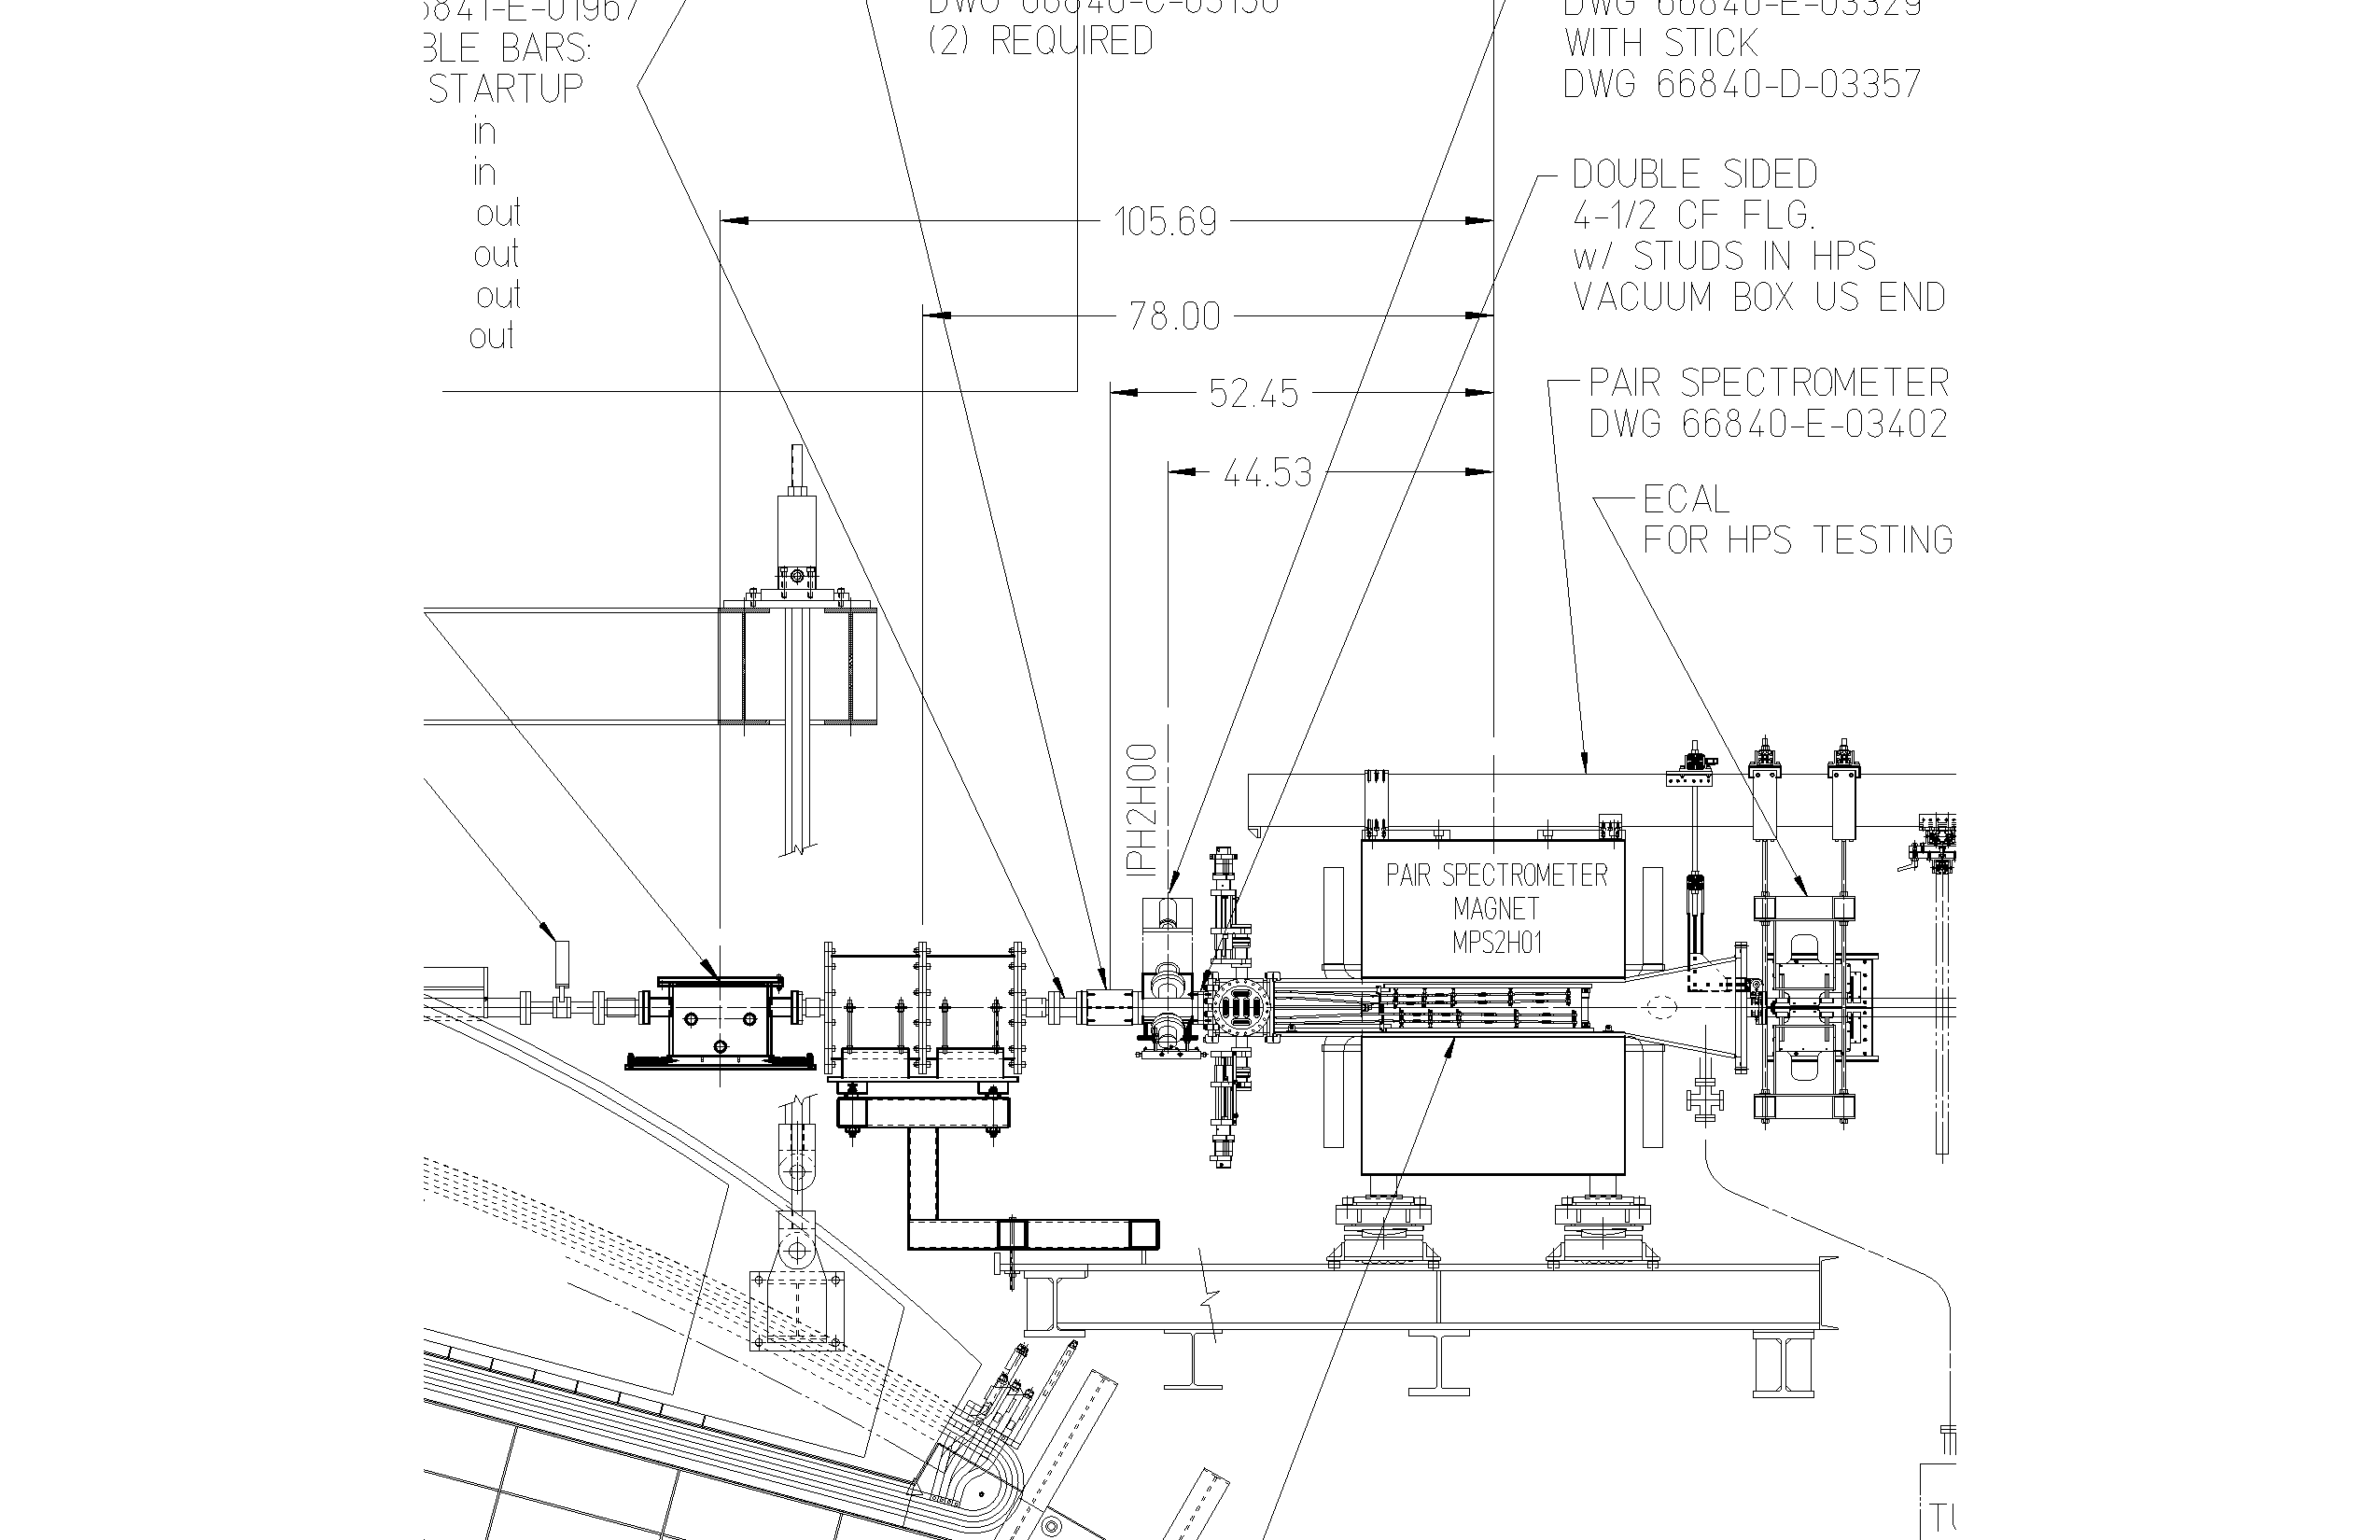
\includegraphics[width=\textwidth]{test2012/HPS_dimensions}
\caption{\small{Layout of the HPS parasitic run.} }
\label{fig:hpstest}
\end{figure}

For the portion of the dedicated HPS run the photon beam was generated in the interaction of the $5.5$ GeV electrons with a gold radiator of $10^{-4}$ r.l., located $\sim 8$ meters upstream of the PS pair converter. After collimation ($D=6.4$ mm), the photon beam passes through the pair converter and through the HPS system. Data were taken on different converters (empty, $1.8\times 10^{-3}$ r.l., $4.5\times 10^{-3}$ r.l., and $1.6\times 10^{-2}$ r.l.). These measurements were repeated for reverse field setting of the pair spectrometer dipole.


\subsubsection{Test Run SVT , {\it Tim}}

The silicon tracking and vertexing detector for HPS Test, or SVT, operates in an existing vacuum chamber inside the pair spectrometer analyzing magnet in Hall B at JLab.  The design principles of the SVT are described in further detail in the HPS Test Run Proposal  \cite{HPS_tPROP}. There are five measurement stations, or ``layers'', placed immediately downstream of the target. Each layer comprises a pair of closely-spaced planes and each plane is responsible for measuring a single coordinate, or ``view''. Introduction of a stereo angle between the two planes of each layer provides three-dimensional tracking and vertexing throughout the acceptance of the detector with one redundant layer. 

In order to accommodate the dead zone, the SVT is built in two halves that are mirror reflections of one another about the plane of the nominal electron beam.  Each half consists of five double-sided modules mounted on a support plate that provides services to the modules and allows them to be moved as a group relative to the dead zone. Each module places a pair of silicon microstrip sensors back-to-back at a specified stereo angle with independent cooling and support.

The vacuum chamber being used for HPS Test cannot accommodate the 90-degree stereo layers planned for the full experiment to optimize the vertex resolution \cite{HPS_PROP}. Instead, 100 milliradian stereo is used in the first three layers to provide higher-resolution 3-d space points for vertexing. The 50 milliradian stereo of the last two layers breaks the tracking degeneracy of having five identical layers and minimizes fakes from ghost hits, improving pattern recognition while still providing sufficient pointing resolution into Layer 3 for robust hit association in the denser environment there. The details of the five layers are shown in Table \ref{tab:trk} and a solid model of the detector layout is shown in Figure \ref{fig:tracker_model}.  Figure \ref{fig:tracker_halves} shows a photograph of both completed detector halves prior to final assembly.  Altogether, this layout comprises 20 sensors and hybrids and 100 APV25 chips for a total of 12780 readout channels. 

\begin{table}[h]
\begin{center}
\begin{tabular}{lccccc}   
\hline \hline 
    Layer & 1 & 2 & 3 & 4 & 5 \\      
\hline
    nominal $z$, from target (cm)  & 10 & 20 & 30 & 50 & 70  \\ 
    Stereo Angle (mrad)  & 100 & 100 & 100 & 50 & 50 \\ 
    Bend plane resolution ($\mu m$)  & $\approx$6 & $\approx$6 & $\approx$6 & $\approx$120 & $\approx$120  \\ 
    Non-bend plane Resolution ($\mu m$)  & $\approx$6 & $\approx$6 & $\approx$6 & $\approx$6 & $\approx$6  \\ 
    \# sensors  & 4 & 4 & 4 & 4 & 4  \\ 
    Nominal dead zone  & $\pm1.5$  & $\pm3.0$  & $\pm4.5$  & $\pm7.5$  & $\pm10.5$  \\ 
    Power consumption & 6.9 & 6.9 & 6.9 & 6.9 & 6.9 \\
\hline \hline
\end{tabular}
\caption[]{Layout of the HPS SVT. }
\label{tab:trk} 
\end{center}
\end{table}

\begin{figure}[ht]
    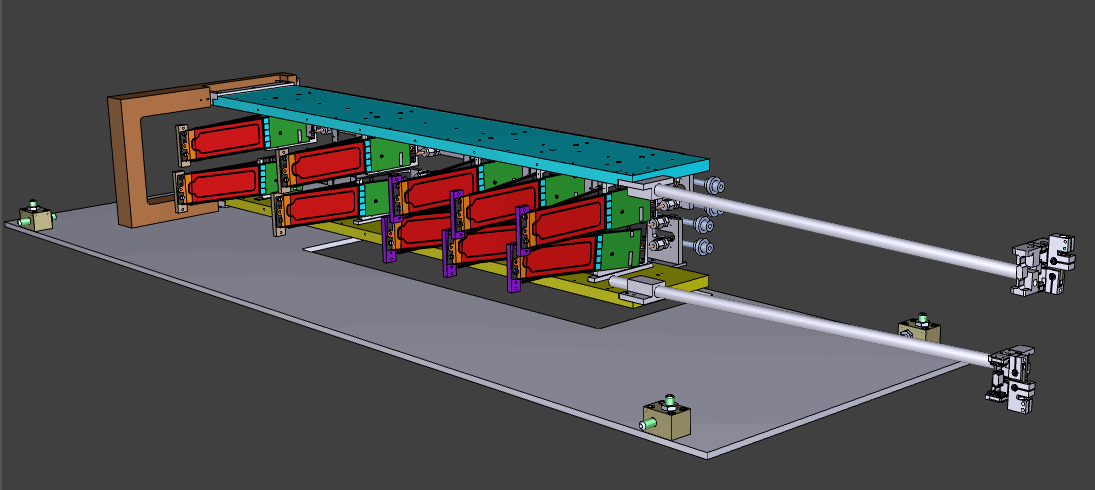
\includegraphics[width=\textwidth]{test2012/HPS_nocables_nowires}
\caption{\small{A partial rendering of the HPS Test SVT solid model showing the modules of the upper and lower half-detectors on their support plates, the hinged C-support, the motion levers, the cooling manifolds on their strain relief plate and the baseplate with its adjusters.  The sensors are shown in red and the hybrids in green. The beam enters from the right.} }
\label{fig:tracker_model}
\end{figure}

\begin{figure}[ht]
    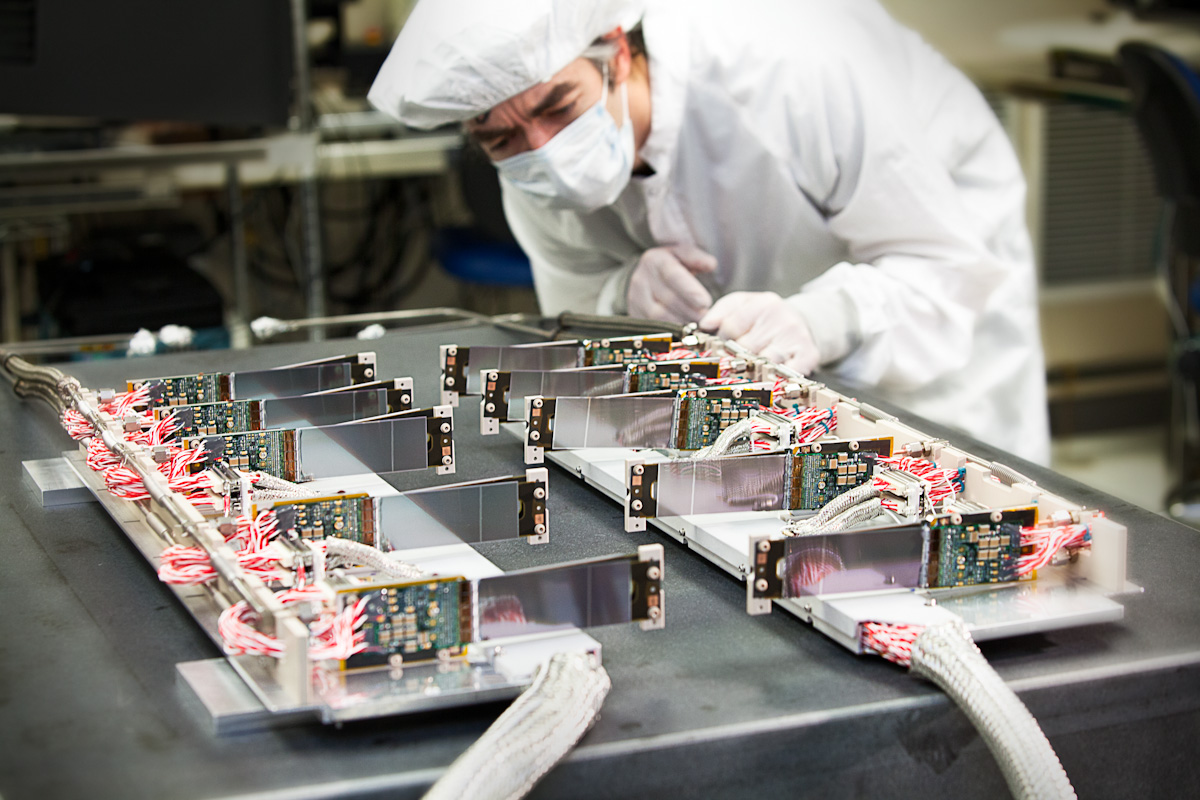
\includegraphics[width=\textwidth]{test2012/2012-101-PHOTON-DETECTOR-001.jpg}
\caption{\small{Both halves of the HPS Test SVT fully assembled at SLAC.} }
\label{fig:tracker_halves}
\end{figure}

Power is provided to each hybrid using CAEN power supplies provided by Fermilab. Three low voltages are supplied for the APV25 and one high voltage to reverse bias the sensor. The supplies that provide sensor bias are capable of 500V operation and can be used to test operation at high voltage in close proximity to an electron beam. The total power consumption of each hybrid during normal operation is about 2 W, which is removed with the cooling system. Care was exercised in selecting power and data cables, to ensure vacuum compatibility and sufficient radiation hardness. The teflon-coated twisted pair copper wires selected are rated for 400kRad, well above the expected exposure of 20kRad/week. A special purpose junction box interfaces the CAEN power supply output channels to the SVT hybrids. Control of the supplies is provided via an EPICS graphical user interface, which allows monitoring of the detector and interlock protection as well.

The linear shifts that define the opening of the SVT are controlled by a pair of stepper motors located in low field regions at the ends of the analyzing magnet.  For photon running, these are locked in the open position, but for electron running they will be connected and controlled through EPICS so that the distance between the beam and the sensors can be adjusted to balance detector occupancies and acceptance.


\subsubsection{Test run ECal {\it Stepan}}

The HPS Test Run electromagnetic calorimeter (ECal) consists of 442 lead-tungstate (PbWO$_4$) crystals with avalanche photodiode (APD) readout, \cite{HPS_PROP_UPD}. 
Crystals in the ECal are arranged in two modules.  There are 5 layers in each module;  four layers have 46 crystals and one has 37.  The ECal is mounted downstream of the analyzing dipole magnet at the distance of $\sim 148$ cm from the upstream edge of the magnet. The two Ecal modules are positioned just above and below the beam plane such that the edge of the crystal closest to the beam is $3.7$ cm from it. As was described in Section \ref{setup} we did not use the vacuum chamber between the two ECal modules for the photon test run, instead 2'' beam pipe was used to transport photon beam from the pair spectrometer vacuum chamber to HDIce target.  

\begin{figure*}[t]
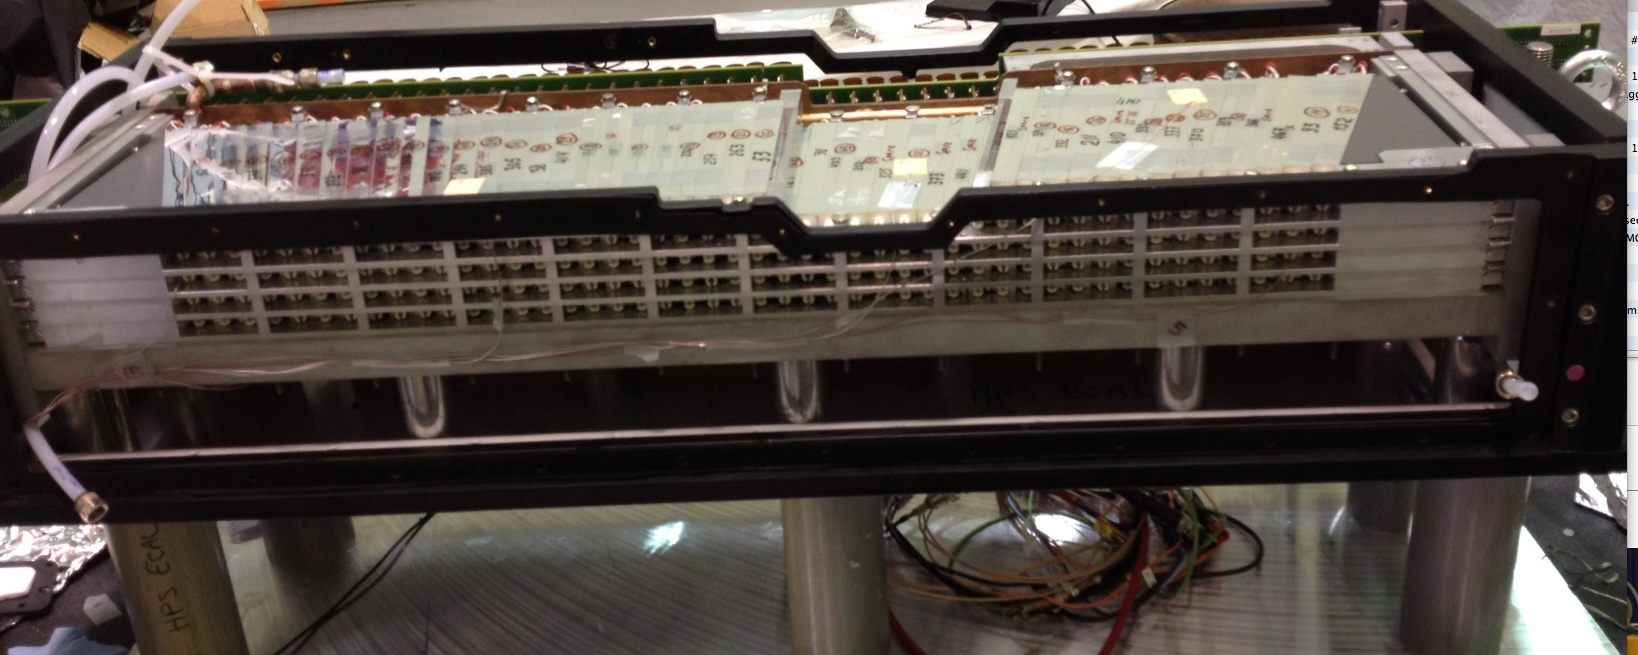
\includegraphics[ scale=0.25]{test2012/ecal_assembly.JPG}
\caption{\small{Assembly of the ECal bottom module.}}\label{fig:ecal_assembly}
\end{figure*}

In order to maintain stable performance of the PbWO$_4$ calorimeter, the crystals and APDs are enclosed within a temperature stabilized environment, held constant at the level of $1~^o$F. The expected energy resolution of the system from operational experience with the IC is $\sigma_E/E \sim 4.5\% / \sqrt{E (GeV)}$. As in the IC, PbWO$_4$ modules are connected to a motherboard that provides power to and transmits signals from individual APDs and pre-amplifier boards. Crystals inside the box are supported by aluminum frames, Figure \ref{fig:ecal_assembly}.

For this run the ECal made use of the existing low and high voltage systems from the CLAS/IC, as well as signal cables and splitters. Connectors on the existing signal cables have been rearranged to accommodate the new layout of the channels. 
 
In Figure \ref{fig:ecal_mounted} ECal is shown in its installed position for the parasitic run with photon beams. It centered relative to the beam that passes in between two parts of ECal through $3$ inch beam pipe. Cooling lines, as well as signal, HV and LV cables are visible. 
 
\begin{figure*}[t]
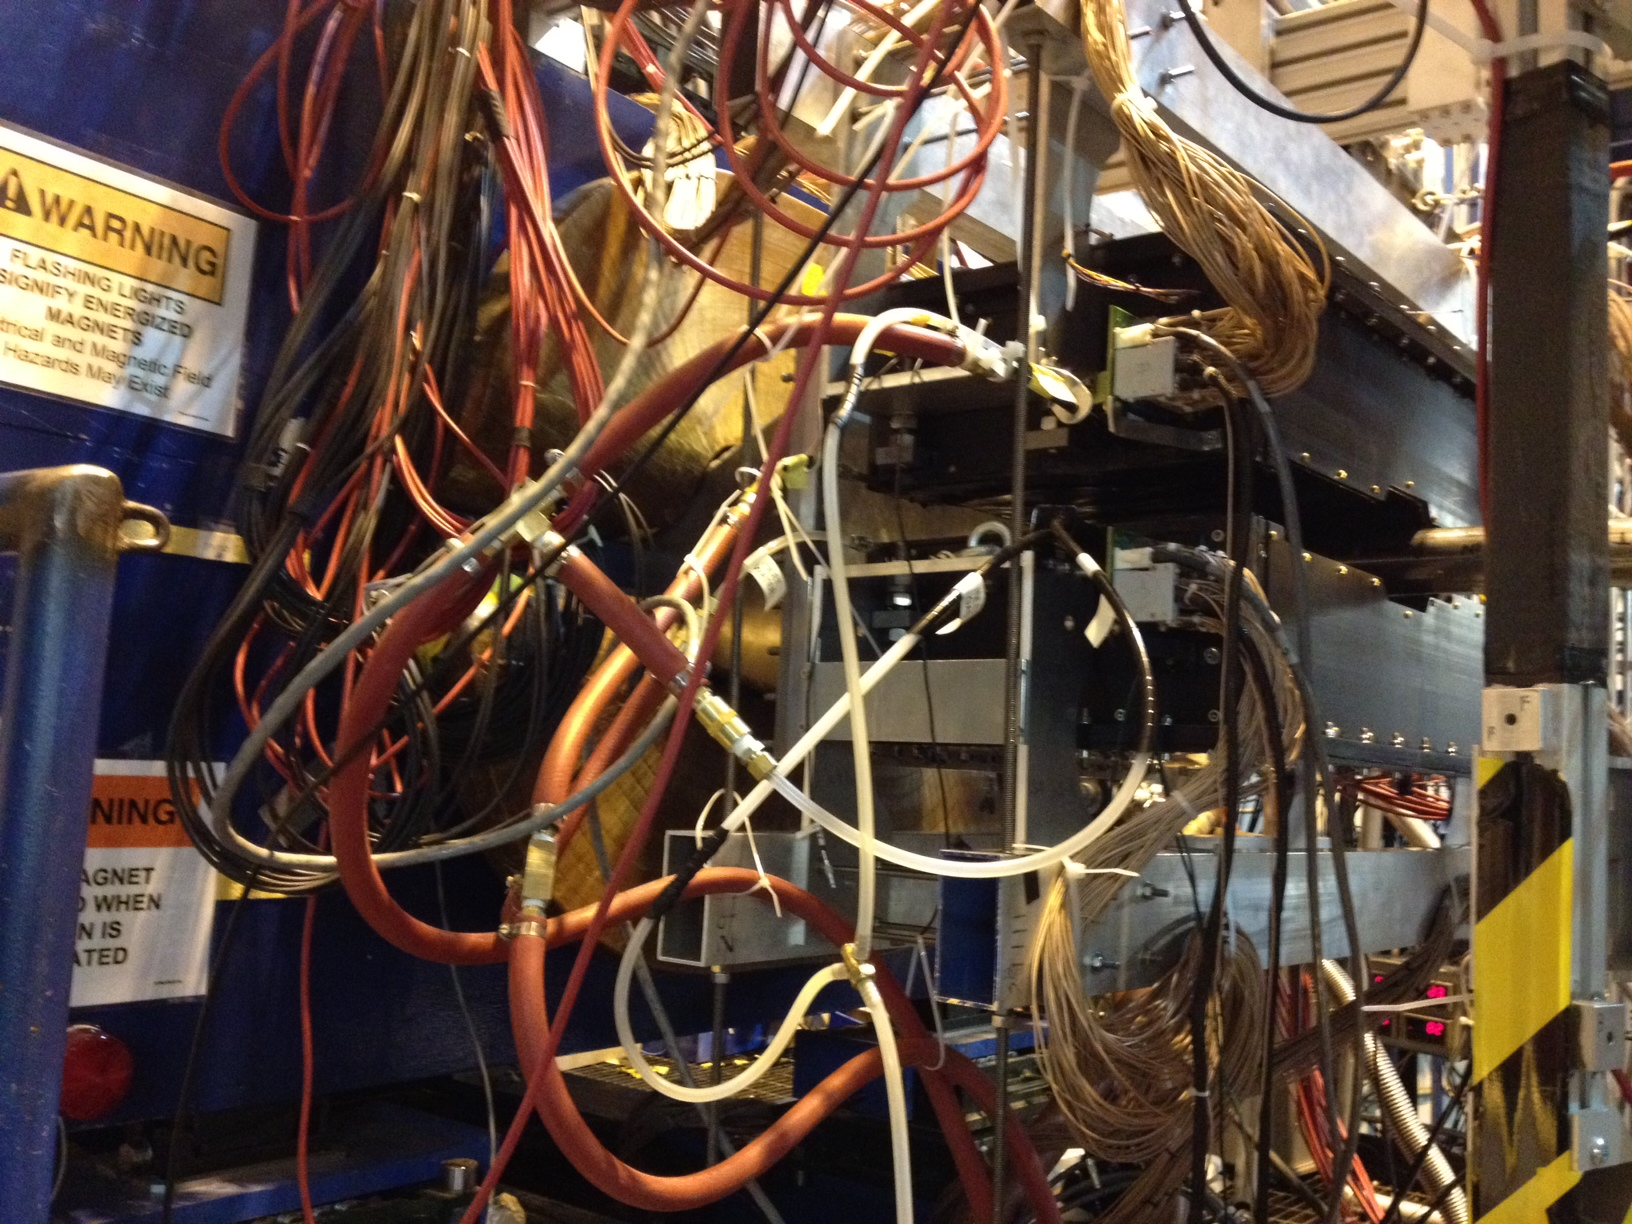
\includegraphics[ scale=0.25]{test2012/ecal_mounted.JPG}
\caption{\small{ECal mounted downstream of the Hall-B pair spectrometer for the parasitic run with photon beams. Hoses for the cooling system, and the power and signal cables for beam-right side of both modules are visible.}}\label{fig:ecal_mounted}
\end{figure*}




\subsection{Test Run Apparatus Performance {\it Pelle}} 

\subsubsection{SVT Performance}
\vspace{1cm}{\bf Calibration [Omar]}


Description of hit amplitude, baseline/gain calibration, noisy channels/chips, pulse shape cuts, occupancy. 

Plots: Response plot, gain, noisy channels vs run nr?, data/MC of noise hits,Data/MC plot of occupancy for some layers  

\vspace{1cm}{\bf Cluster reconstruction [Omar]}


Description of the cluster reconstruction.

Plots: mip distribution

\vspace{1cm}{\bf SVT timing [Sho]}

The time reconstruction algorithm described in \ref{sec:svtŧ} was used to fit a single hit to each SVT channel in each event.
Pileup was not considered due to the very low hit rate in the SVT.

As shown in Figure \ref{fig:apvfit}, values of fit $\chi^2$ fell in the distribution of $\chi^2$ for 4 degrees of freedom (6 points -- 2 fit parameters).

\begin{figure}[ht]
	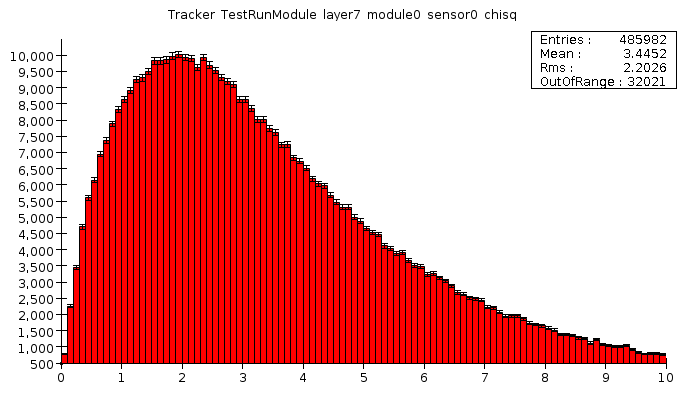
\includegraphics[width=\textwidth]{test2012/svtperformance/apvfit_chisq}
	\caption{\small{Histogram of $\chi^2$ values for pulse fits for all channels on a representative sensor. Peak at 2 is consistent with dof of 4, as expected.} }
	\label{fig:apvfit}
\end{figure}

After clustering these hits, the hit time for the cluster is computed as the amplitude-weighted average of the channel hit times. 



Since we have no measurement of the ``true'' hit time, we use the average of all cluster times in a track as the ``track time,'' and take the residual of the cluster time relative to that.
The track time, shown in Figure \ref{fig:tracktime}, has the expected amount of trigger jitter.
Different sensors have systematic offsets in hit time (up to a couple ns) due to time of flight and variations between readout chips. 
We correct these offsets so that the time residual is centered around 0 for each sensor. The RMS of the residual (from a Gaussian fit to the residual histogram, Figure \ref{fig:timeres}) is roughly 2.4 ns for each sensor.

\begin{figure}[ht]
	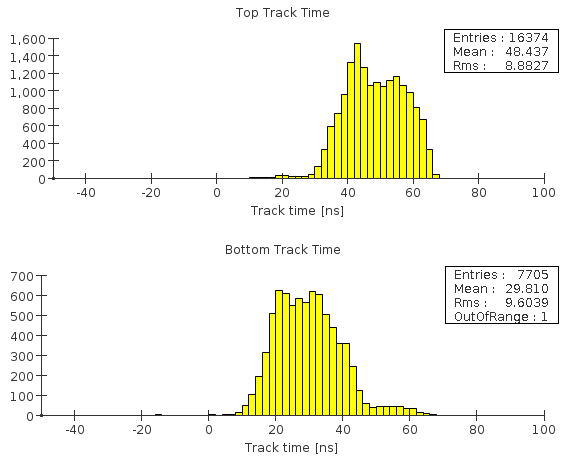
\includegraphics[width=\textwidth]{test2012/svtperformance/track_time}
	\caption{\small{Track time distribution, measured relative
	to the APV25 clock, for top and bottom tracks. The
width of the distribution is due to trigger jitter (24 ns
jitter in tracker readout clock, plus 16 ns jitter in the
trigger system). The shift between top and bottom
is due to a trigger time shift between the two halves
of the ECal.} }
	\label{fig:tracktime}
\end{figure}


Because the track time is calculated using the individual hit times, the hit time is positively correlated with the track time; thus the RMS of the residual is slightly smaller than the true time resolution.
The standard deviation of this residual for $n$-hit tracks where all hits have the same time resolution is reduced by a factor of $\sqrt{(n-1)/n}$; since most of our tracks have 8 clusters, the true time resolution is 2.6 ns. 

\begin{figure}[ht]
	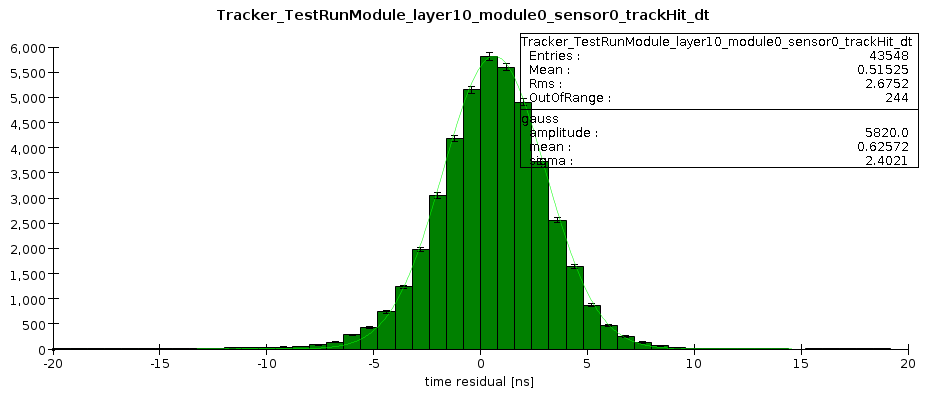
\includegraphics[width=\textwidth]{test2012/svtperformance/timeres}
	\caption{\small{Histogram and Gaussian fit of residual of cluster times for a representative sensor, relative to the track time. Because the cluster times and track time have positive covariance, the true time resolution is slightly larger than the standard deviation shown here.} }
	\label{fig:timeres}
\end{figure}

%\begin{figure}[ht]
%	\includegraphics[width=\textwidth]{test2012/svtperformance/hit_dt}
%	\caption{\small{} }
%	\label{fig:hit_dt}
%\end{figure}

This is somewhat worse than the $\approx 2$ ns resolution expected, but we believe this discrepancy is due to our fit function. Our pulse shape fit assumes an ideal CR-RC pulse shape; since the actual pulse shape has a slower rise time, there is a systematic pull on the hit time when a hit comes immediately before the APV clock time. 
This is visible in Figure \ref{fig:timeres_2D} as a shift in the residual at certain values of track time.
Work is in progress to use the actual pulse shape in time reconstruction; this should improve time resolution.

\begin{figure}[ht]
	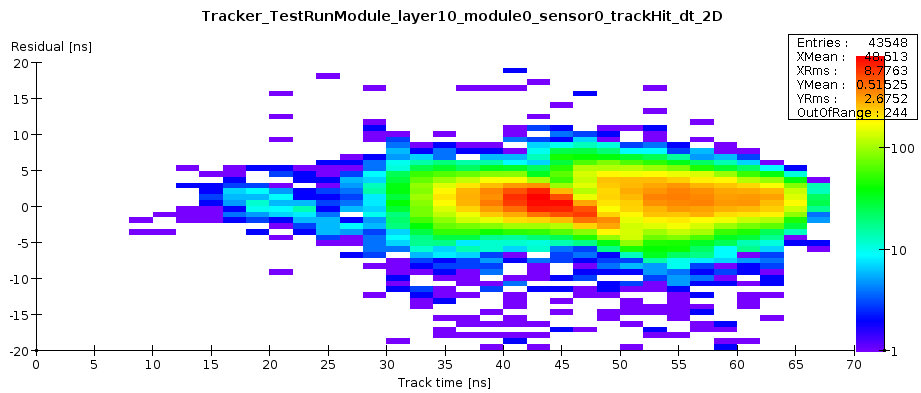
\includegraphics[width=\textwidth]{test2012/svtperformance/timeres_2D}
	\caption{\small{Plot of the time residual for a representative sensor vs. the track time. 
		The kinks in the horizontal band are caused by the fitter; without them the 1-D histogram in Figure \ref{fig:timeres} (the projection of this histogram) would be narrower.} }
	\label{fig:timeres_2D}
\end{figure}

\vspace{1cm}{\bf Tracking algorithms [Matt/Omar]}


Pattern recognition/Stereo hit reconstruction and description of the tracking algorithm. 

Plots: tracking efficiency vs run nr, hit efficiency vs run nr for data. Overlay MC.

\vspace{1cm}{\bf Two track events analysis [Matt]}

Analysis of two track events. 

Plots: invariant mass, vertex position, 2-track event multiplicity. Compare with MC for all these 


\vspace{1cm}{\bf SVT DAQ Performance [Pelle/Omar/Ryan]}
General discussion on SVT rates, event size.

Plots: 

\label{sec:svtperformance}

%\subsubsection{Alignment of the SVT}
%\label{sec:alignment}
\vspace{1cm}{\bf Alignment of the SVT [Pelle]}
%Good alignment of the SVT is critical to achieving the expected tracking performance and physics reach. 
%The sensors must be aligned internally and with respect to the target and other beam line components for optimal performance. 
%The alignment of the test run apparatus proceeds in several steps which must be tied together to achieve the final alignment.
%These include survey measurements of various SVT assemblies, a beam line survey at JLab, and finally 
%a track-based alignment. 

The SVT was aligned using a combination of optical, laser and touch probe surveys at SLAC and JLab. The 
optical survey of individual modules with precision of a few microns are combined with a touch-prove survey 
of the overall SVT support structure, with 25-100 microns precision, to locate the silicon sensor layers with 
respect to the support plates and the mechanical survey balls on the base plate.
%Mechanical surveys using touch probes was performed on the two SVT tracker planes before 
%shipping to JLab. This survey measured reference points on the base plate, C-support and on the surface of the tracker support plates. These positions where then tied to very precise optical survey of each sensor module, referencing the silicon sensor position w.r.t. to the cooling blocks. 
%An important aspect of the mechanical survey is the relatively large sag of 
%the 70~cm long support plate which is supported by the C-support hinge on one end and the 
%extension bar attached to the linear shaft at the other. The measured sag without all services 
%(cooling manifold and cables was not dressed at this point) was more than $250~\mu$m.  
%For HPS, only the first three layers are being supported from each end which will reduce this 
%sag with at least a factor of four. {\color{red} check this}. The goal of the mechanical surveys is 
%to reach a relative alignment of the 
%silicon to about $100-200~\mu$m where alignment using tracks become feasible and the 
%improvements from mechanical surveys become harder. 
After full assembly and installation of the SVT at JLab, a mechanical survey of the SVT base plate position 
inside the pair spectrometer vacuum chamber is used to determine the global position of the SVT with respect 
to CEBAF beam line. 
%at the as-built alignment.  The sag
%of the long support plates and lever arms used in the test run are the dominant error in determining
%relative modules positions, a defect addressed in the proposed design for the SVT.
%Finally at JLab, with a fully assembled 
%tracker, an optical and touch probe survey was performed to locate 
%the SVT inside the vacuum chamber, using the measurements of the base plate, in the reference coordinate system of 
%the analyzing magnet. 
The resulting survey-based alignment has the position of the silicon sensors correct to within a few hundred 
microns as shown in the reconstructed track residuals in Fig.~\ref{fig:res_top}. 
%This level of internal alignment 
%shows that the survey approach, while not perfect, is adequate as a starting point to bootstrap the SVT 
%alignment. 
%At this level of internal 
%alignment   an internal SVT alignment with track residuals less than a few 
%hundred microns shown in .  is then studied using reconstructed tracks in the SVT. The main observable of the internal alignment of the silicon 
%sensors is the so-called track residual. It is 
%defined as the difference of the measured and predicted track 
%position at that sensor. Figure~\ref{fig:res_top} 
%shows representable 3D space point track residuals, relative to track parameters determined at the target, for tracks reconstructed in the top half of the tracker.
\begin{figure*}[]
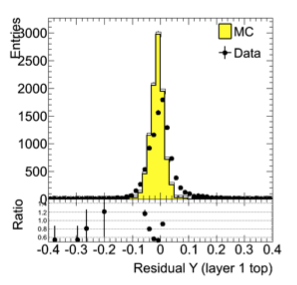
\includegraphics[ scale=1.2]{test2012/alignment/pictures/res_top/res_top-1.png}
%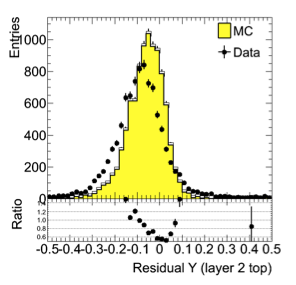
\includegraphics[ scale=0.5]{test2012/alignment/pictures/res_top/res_top-2.png}
%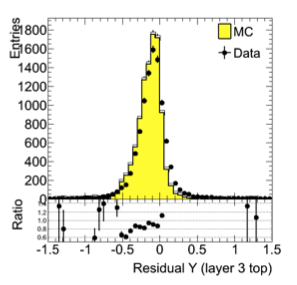
\includegraphics[ scale=0.5]{test2012/alignment/pictures/res_top/res_top-3.png}
%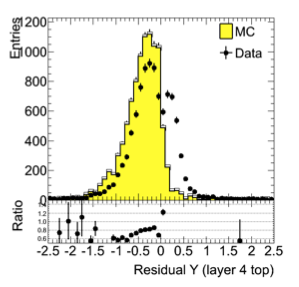
\includegraphics[ scale=1.2]{test2012/alignment/pictures/res_top/res_top-4.png}
%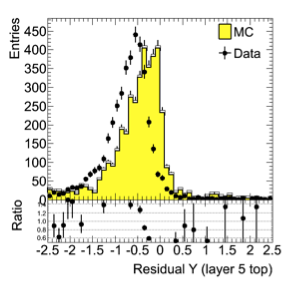
\includegraphics[ scale=0.5]{test2012/alignment/pictures/res_top/res_top-5.png}
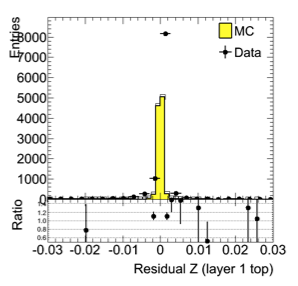
\includegraphics[ scale=1.2]{test2012/alignment/pictures/res_top/res_top-6.png}
%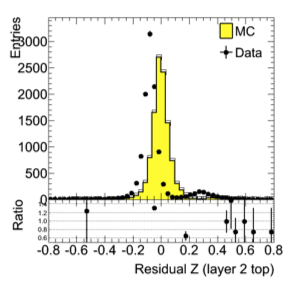
\includegraphics[ scale=0.5]{test2012/alignment/pictures/res_top/res_top-7.png}
%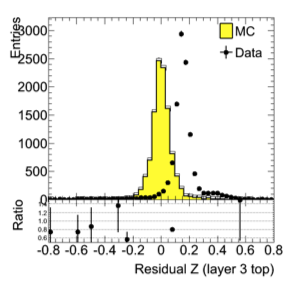
\includegraphics[ scale=0.5]{test2012/alignment/pictures/res_top/res_top-8.png}
%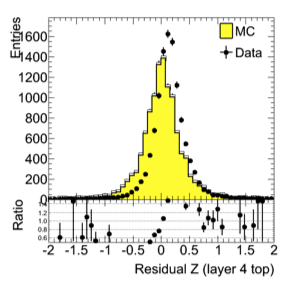
\includegraphics[ scale=1.2]{test2012/alignment/pictures/res_top/res_top-9.png}
%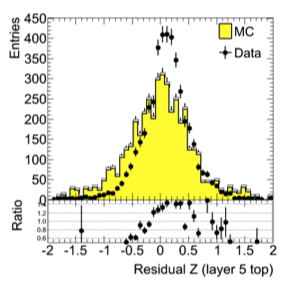
\includegraphics[ scale=0.5]{test2012/alignment/pictures/res_top/res_top-10.png}
\caption{\small{Residual between the actual hit position and the predicted position in layer 1 from the reconstructed tracks in the bend (left) and non-bend (right) plane in the top half of the SVT after mechanical survey. The filled histogram show the predicted residual for simulated events with an ideal geometry. The X-scale is in mm.}}
\label{fig:res_top}
\end{figure*}
%These are compared to the residuals from an ideally aligned tracker with residuals centered at zero.
%Note the larger width for the downstream layers,highlighting the large 
%multiple scattering contribution in the track reconstruction. 
%The intrinsic single hit resolution of $\approx 6~\mu$m is negligible for layers beyond the second. 
%Fig.~\ref{fig:res_top_summary} shows a summary of the mean residuals for each layer of the tracker 
%after the mechanical survey alignment constants have been applied.
%\begin{figure*}[t]
%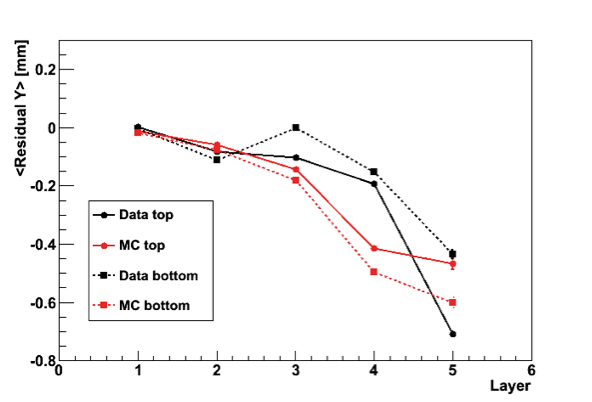
\includegraphics[ scale=0.7]{test2012/alignment/pictures/res_top/res_top_summary-1.png}
%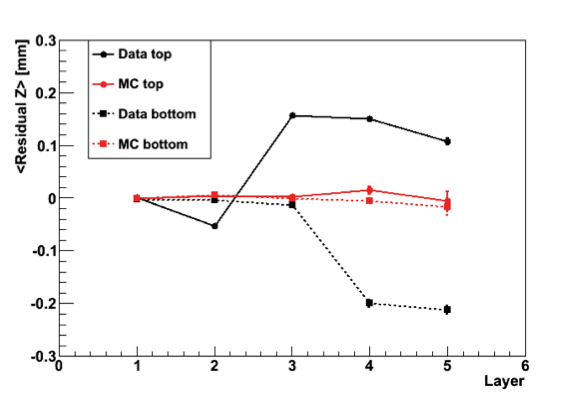
\includegraphics[ scale=0.7]{test2012/alignment/pictures/res_top/res_top_summary-2.png}\caption{\small{Mean of the track residuals for each detector layer in the top tracker half 
%in the bend (left) and non-bend (right) plane after mechanical survey constants are applied.}}\label{fig:res_top_summary}
%\end{figure*}
%Note that these pull distributions come from biased 
%residuals (the hit was used in the track fit) and are thus not expected to have a 
%width of one. 
%\begin{figure*}[]
%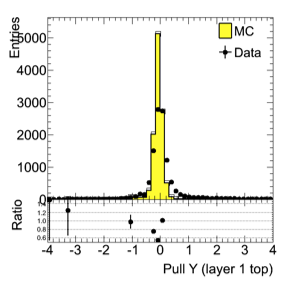
\includegraphics[ scale=1.2]{test2012/alignment/pictures/res_pull_top/res_pull_top-1.png}
%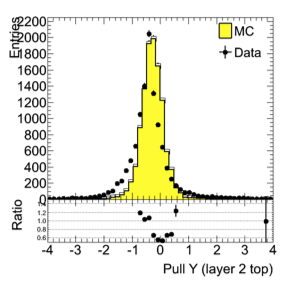
\includegraphics[ scale=0.5]{test2012/alignment/pictures/res_pull_top/res_pull_top-2.png}
%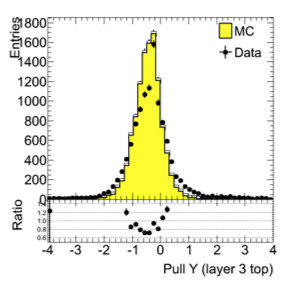
\includegraphics[ scale=0.5]{test2012/alignment/pictures/res_pull_top/res_pull_top-3.png}
%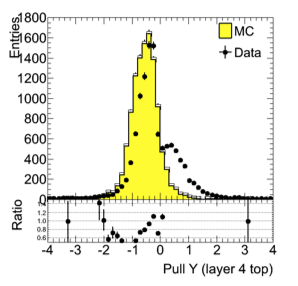
\includegraphics[ scale=1.2]{test2012/alignment/pictures/res_pull_top/res_pull_top-4.png}
%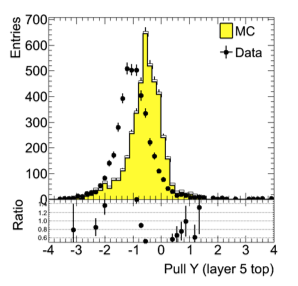
\includegraphics[ scale=0.5]{test2012/alignment/pictures/res_pull_top/res_pull_top-5.png}
%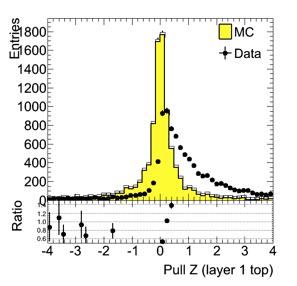
\includegraphics[ scale=1.2]{test2012/alignment/pictures/res_pull_top/res_pull_top-6.png}
%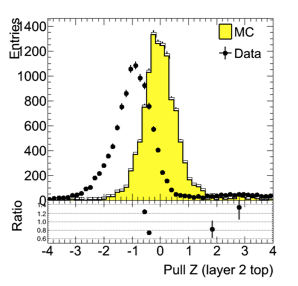
\includegraphics[ scale=0.5]{test2012/alignment/pictures/res_pull_top/res_pull_top-7.png}
%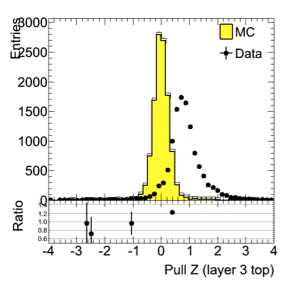
\includegraphics[ scale=0.5]{test2012/alignment/pictures/res_pull_top/res_pull_top-8.png}
%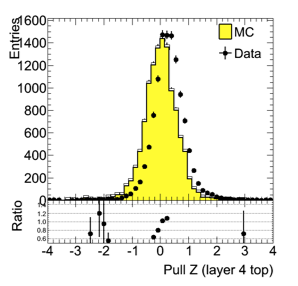
\includegraphics[ scale=1.2]{test2012/alignment/pictures/res_pull_top/res_pull_top-9.png}
%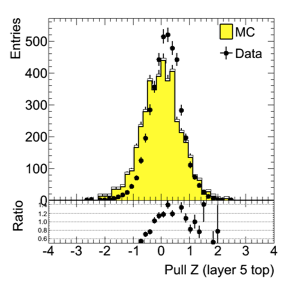
\includegraphics[ scale=0.5]{test2012/alignment/pictures/res_pull_top/res_pull_top-10.png}
%\caption{\small{Track residual pulls in the bend (top) and non-bend (bottom) plane 
%for tracks reconstructed in the 
%top half of the tracker.  }}
%\label{fig:res_pull_top_nonbend}
%\end{figure*}

%In electron running, the beam spot can be used as a constraint in the global track-based alignment. 
We also extrapolate the reconstructed tracks back to the converter located $\approx 77$~cm 
from our first silicon layer to understand the tracker alignment w.r.t. to the other components on the 
beam line. Figure~\ref{fig:extrapol_converter} shows good agreement of the reconstructed track position at the converter with that predicted from simulation using the measured field map of the analyzing magnet to take into account the fringe field. The offset of the horizontal position simply reflects the fact that the positions are reconstructed in an SVT-centered coordinate system, which is tilted with respect to the beam coordinate system.
\begin{figure*}[t]
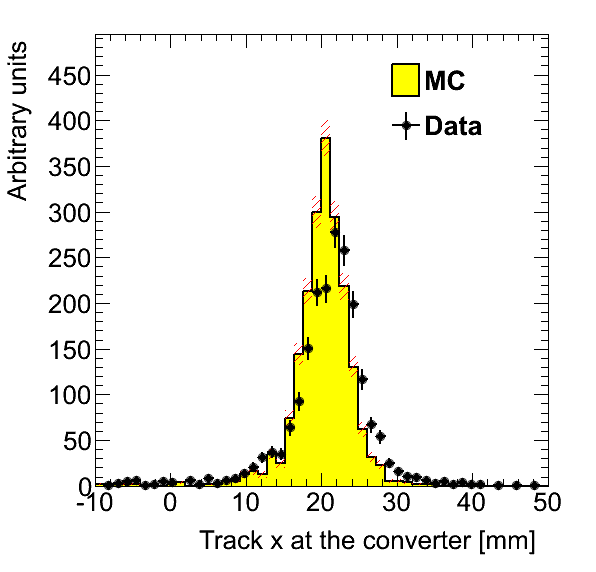
\includegraphics[ scale=0.25]{test2012/alignment/pictures/extrapolation_converter/h_trk_top_fr_conv_y_h_trk_top_conv_y_dataMC_twotrksel.png}
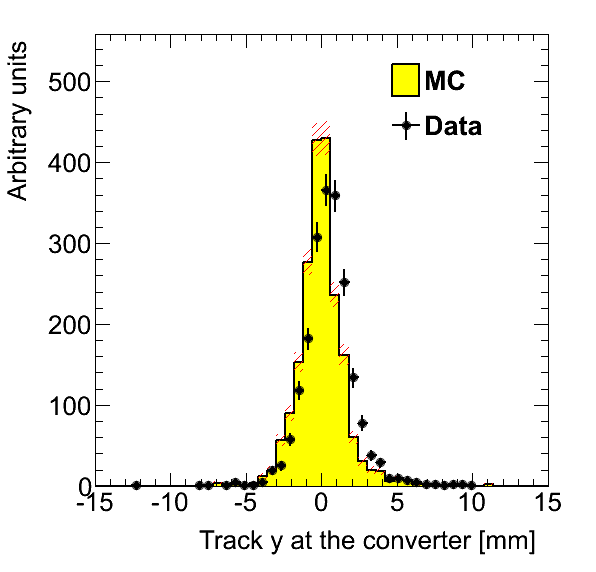
\includegraphics[ scale=0.25]{test2012/alignment/pictures/extrapolation_converter/h_trk_top_fr_conv_z_h_trk_top_conv_z_dataMC_twotrksel.png}
%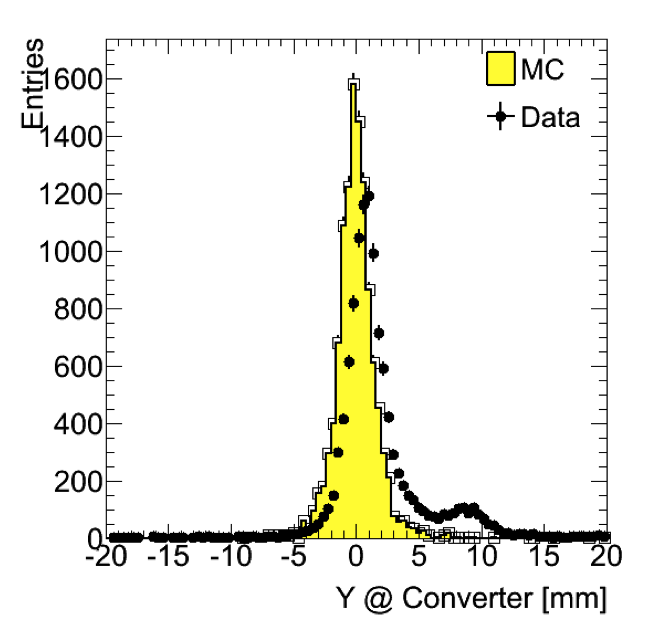
\includegraphics[ scale=0.5]{test2012/alignment/pictures/extrapolation_converter/extrapolation_Y_converter_top.png}
%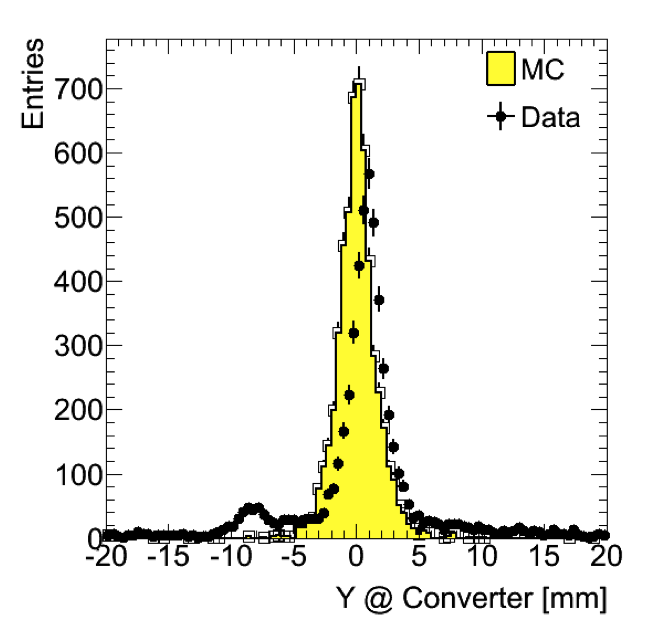
\includegraphics[ scale=0.5]{test2012/alignment/pictures/extrapolation_converter/extrapolation_Y_converter_bot.png}
\caption{\small{Extrapolated track positions for reconstructed e$^{+}$e$^{-}$ pairs in the SVT taking into account the measured fringe field of the analyzing magnet. 
The filled histograms show the prediction from simulation using an ideal geometry. 
A shift in the bend-plane coordinate for tracks in the bottom half (top right) is likely due to alignment or incomplete description of the
magnetic field at the edge of the magnet.
%The extra bumps in the data at $\pm10$~mm arise from backgrounds originating upstream of the 
converter.
}}
\label{fig:extrapol_converter}
\end{figure*}
%The width is roughly consistent with between data and simulation with a shift in the bend-plane 
%coordinate for tracks in the bottom half which is likely due to alignment or incomplete description of the 
%magnetic field at the edge of the magnet. 
%There are two small bumps in the vertical position in the data arising from backgrounds 
%originating upstream of the converter verified using the run without a converter.
%The luminous region, inferred from harp scans of the photon beam profile, has a width of about 1~mm 
%%(best described by a double Gaussian: $0.71e^{\frac{x}{0.366}}\times 0.29e^{\frac{x}{1.111}}$)
%and a total beam envelope of around 7~mm. The small bumps in data at $\pm10$~mm 
%are from particles produced upstream of the converter. The width and position of the tracks 
%are roughly consistent with the expected distribution from an ideal geometry as shown by the simulated 
%tracks in the same figures. The larger shift in the bend direction for bottom tracks 
%is still under investigation. 

With initial residuals less than $\sim 500~\mu$m across all layers of 
the tracker and a reconstructed beam profile similar to that expected from simulation, it appears these survey techniques 
are adequate to bootstrap the SVT alignment. 
For HPS, we are developing a more sophisticated global track-based alignment technique to reach 
the final alignment precision. This framework will also enable us to explore and understand important details 
such as weak modes and how dedicated alignment runs 
(e.g. with magnetic field off or with different targets) may shape operational procedures during HPS running.
%Fig.~\ref{fig:test_harpscan} shows a HARP scan taken during the test run. 
%\begin{figure*}[t]
%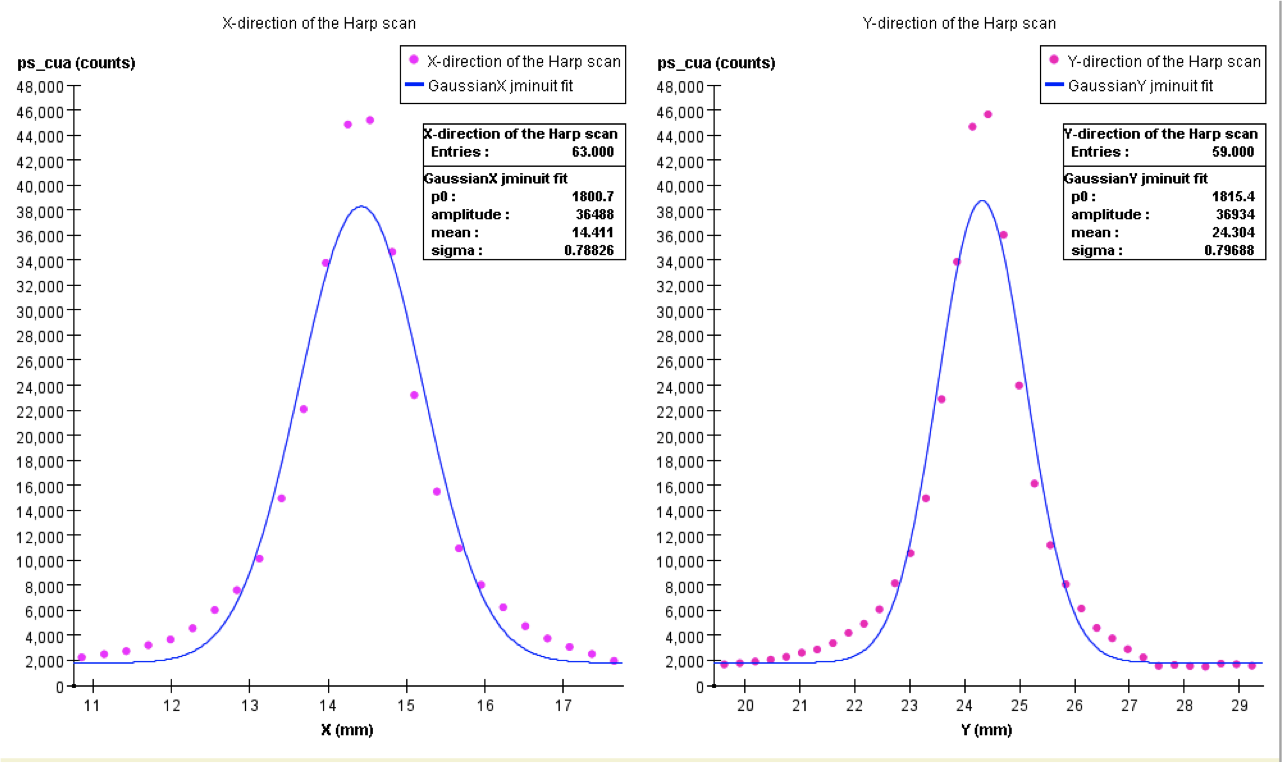
\includegraphics[ scale=0.5]{test2012/alignment/pictures/harp_scan_testrun.png}
%\caption{\small{Photon beam profile HARP scan close to the converter.}}\label{fig:testrun_harpscan}
%\end{figure*}
%The width of the beam can be described by a double Gaussian $0.71e^{\frac{x}{0.366}}\times 0.29e^{1.111}$ which is also used in the simulations. The beam envelope extends out to 
%about 7mm. 


\subsubsection{ECal \& Trigger Performance}

\vspace{1cm}{\bf ECal performance [Sho]}

The ECal preamplifiers shape the APD signal into a CR-RC pulse of rise time $\approx 14$ ns; this is sampled every 4 ns and stored in a pipeline on the FADC readout board.
On receiving a trigger, the FADC searches for rising threshold crossings in the pipeline, and integrates pulses by summing 5 samples before and 30 samples after each threshold crossing.

The noise and pedestal of the readout chain are calibrated by running the ECal readout in a mode where the preamplifier output is sampled every 4 ns in a time window of 100 samples; by looking at a part of the window before the hit, we calibrate the readout channel.

Of 442 crystals/channels, 39 were disabled or disconnected and were not read out by the DAQ. 
13 of these were not read out because of a shortage of FADC readout boards.
The remainder either had no HV bias on the APD, or were disabled in the FADC software due to noise.

In the data, we identified two types of abnormal channels. 
One FADC was not sending trigger signals correctly, resulting in low efficiency. This affected the 13 channels read out by that FADC.
5 channels were diagnosed as noisy because they had a high incidence of hits out of coincidence with the trigger.

A large number of channels were originally misidentified as noisy because they had much higher hit occupancy than neighboring channels.
Gain calibration (described in the next section) shows that these channels have high gain (and thus lower energy threshold) but are otherwise normal.

The abnormal channels were ignored in analysis in order to simplify comparison with Monte Carlo. This leaves 385 useful channels---87\% of the ECal.

We found that one quadrant of the ECal had been miswired in such a way as to flip the horizontal coordinate---the column of crystals nearest the center was connected to the readout channels for the rightmost column, and vice versa.

\begin{figure}[ht]
	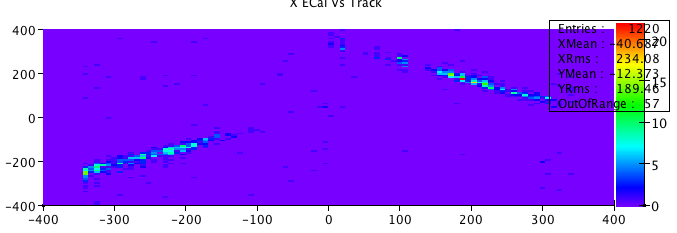
\includegraphics[width=\textwidth]{test2012/ecalperformance/x_match_flip}
	%\includegraphics[width=0.4\textwidth]{test2012/ecalperformance/crystal_edges_flip}
	\caption{\small{ECal hit position from track extrapolation vs. ECal hit position from ECal (for top half of ECal only). Shows that $x>0$ quadrant is flipped.}}
	\label{fig:x_flip}
\end{figure}

\begin{figure}[ht]
	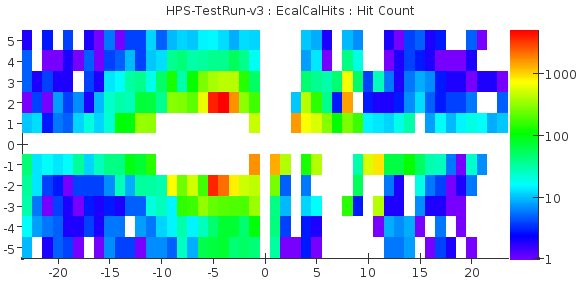
\includegraphics[width=0.5\textwidth]{test2012/ecalperformance/hitrates}
	\caption{\small{Hit rates (above an energy threshold, to cut out effect of gain variations) vary smoothly with position.}}
	\label{fig:hitrates}
\end{figure}

For ECal analysis, cluster reconstruction was done using the algorithm described in \cite{HPS_PROP}: build clusters around seed hits (hits above a ``seed'' energy threshold and with greater energy than any neighboring hits), and add all neighboring hits above an ``add'' energy threshold.

\vspace{1cm}{\bf ECal Calibration [Sho]}

We calibrate gain of the individual ECal channels using the SVT measurement of track momentum. 
The ratio of cluster energy to track momentum is calculated both for Monte Carlo simulation and test run data at each point in the ECal, and we find the value of gain for each channel that brings the two into agreement.

We use a formula to compute the ``weighted E/p'' for a crystal, representing the average E/p for clusters that include the crystal: $\frac{\sum_j w_{j,i}}{\sum_j\frac{P_j}{E_j}w_{j,i}}$.
We disable all SVT and ECal channels in the simulation that were inoperable or noisy in the test run, so any efficiency or bias effects that affect the real data should be reflected in the simulation as well.

The calibrated gains are corrected by the ratio between the weighted E/p values from Monte Carlo and real data.
The E/p in Monte Carlo data is also affected by the gain because the trigger thresholds change, so both Monte Carlo and data reconstruction are rerun with each iteration of gain calibration.
It takes up to 4 iterations for the gains to stabilize; the final values are shown in Figure \ref{fig:gains}.

\begin{figure}[ht]
	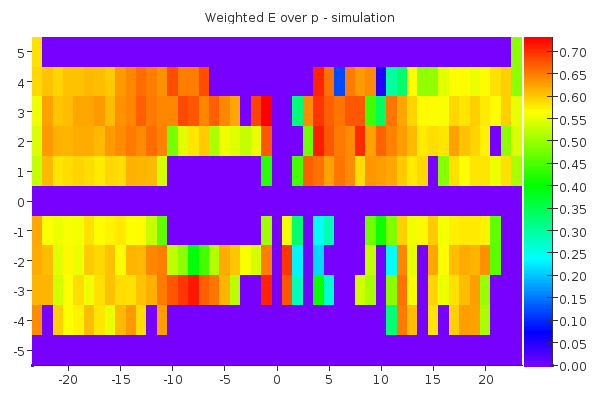
\includegraphics[width=0.45\textwidth]{test2012/ecalperformance/ecalgainplots_corr_sim}
	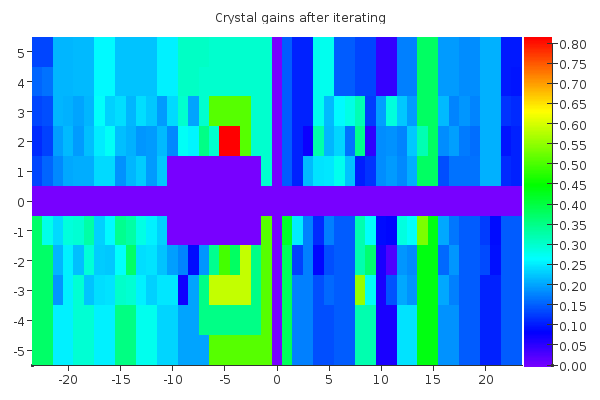
\includegraphics[width=0.45\textwidth]{test2012/ecalperformance/gains}
	\caption{\small{Weighted E/p from Monte Carlo simulation (left), calibrated values of gain in units of MeV per ADC count (right).}}
	\label{fig:gains}
\end{figure}

These gains can then be used to convert from ADC counts in a channel to energy deposited into that ECal crystal.
The other information needed to find the energy of an incident particle is the sampling fraction---the ratio of energy read out from crystals to energy of an incident particle.
The conventional sampling fraction---the fraction of incident energy that is deposited in crystals---is approximately 0.9 for our ECal, and less at edges.
For our readout, there is additional energy lost because crystals under the readout threshold are not read out.
The weighted E/p used in calibration (see Figure \ref{fig:gains}) is an approximate measurement of sampling fraction, but the sampling fraction is energy-dependent because of the effect of readout threshold.

\vspace{1cm}{\bf Trigger performance [Sho/Ben]}

%\begin{figure}[ht]
%	\includegraphics[width=\textwidth]{test2012/ecalperformance/trigtimes}
%	\caption{\small{}}
%	\label{fig:trigtimes}
%\end{figure}

As described in Section \ref{sec:tesrun_trigger}, the trigger and DAQ integrate pulses differently to measure hit energy. The trigger integrates using a time-over-threshold window, and the DAQ readout integrates using a constant window (5 samples before and 30 samples after a threshold crossing). 

For every event, the trigger reports as a bitmask the trigger decision (top trigger, bottom trigger, or both) and the time the trigger fires.

We study trigger performance by simulating the trigger for each event and comparing actual To study trigger performance, we first convert from readout hits (constant integration window) to trigger hits (time-over-threshold integration). 
This is done by converting from the readout hit to pulse amplitude, then applying the time-over-threshold algorithm to the simulated ECal pulse shape. 
We then simulate the CTP clustering algorithm and the trigger decision (described in Section \ref{sec:tesrun_trigger}), and compare the trigger decision and trigger time reported by the simulation to what was reported by the real trigger.

To eliminate trigger bias in checking the trigger decision, we use a tag and probe method: to check trigger performance in one half of the ECal, we tag events where there was a trigger in the other half, and exactly one probe cluster in the ECal half under test. 
We then measured trigger efficiency (proportion of tagged events where there was a trigger) as a function of ADC counts and energy of the probe cluster.

These turn-on curves are shown for the top half of the ECal in Figure \ref{fig:turnon}. 
The trigger threshold is seen to be 1280 ADC counts as expected; the threshold is not perfectly sharp in this analysis because of uncertainties in the conversion from constant-window to time-over-threshold integrals, but based on comparisons with Monte Carlo simulation we believe the trigger worked exactly as specified. 
The trigger threshold in terms of cluster energy is very uneven for two reasons: gain variations between different ECal crystals lead to threshold variations, and the nonlinearity of the time-over-threshold integral means that the effective threshold is higher for clusters that span multiple crystals.

\begin{figure}[ht]
	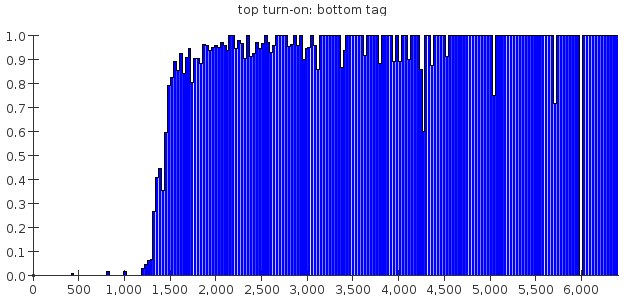
\includegraphics[width=0.4\textwidth]{test2012/ecalperformance/top_turnon_adc}
	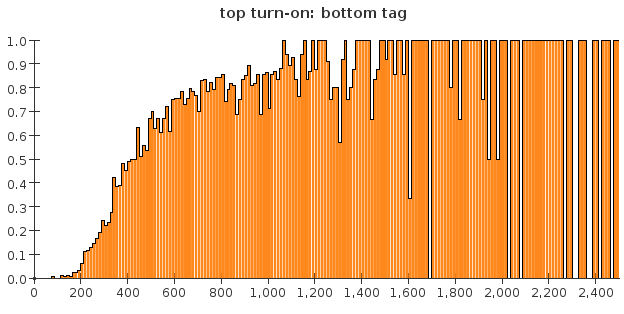
\includegraphics[width=0.4\textwidth]{test2012/ecalperformance/top_turnon_e}
	\caption{\small{Trigger turn-on as a function of probe cluster ADC counts (left) and probe cluster energy in MeV (right). Both plots are for the top half of the ECal; bottom is similar. 
	Energy is not corrected for sampling fraction.}}
	\label{fig:turnon}
\end{figure}

Overall the trigger appears to have functioned exactly as intended. Changes planned for the next run (constant integration window and per-crystal gain calibration constants for the trigger) will solve both of the issues that led to threshold variations in the test run.

What were the rates, lessons learned?

Plots: rates vs time {\it Ben/Sho/Pelle}



\label{sec:ecalperformance}

\subsubsection{Multiple Coulomb Scattering Measurement}
Occupancies close to the beam create many of the key challenges in the HPS experiment
and determine the limits of sensitivity to low A$^\prime$ masses.
These occupancies are dominated by electrons which have multiple Coulomb scattered to relatively large angles in the converter. Because HPS is sensitive to scattering angles far out on the tail of the multiple Coulomb scattering distribution, well beyond the angles important in other experiments, care must be taken
to ensure our simulations are correct in this regime.  In particular,
Geant4 overestimates the multiple Coulomb scattering rate by a factor of two  
at large angles as explained in detail in the appendix (see Fig.~\ref{appendix:2}).
One of the main goals of the test run in 2012 was to evaluate the description of the tails of the multiple Coulomb scattering in order 
to gain further confidence in our expected detector occupancy. As will be shown below, data from the 
test run can be used to confirm our model of multiple Coulomb scattering despite the fact that 
all data was taken with a photon beam.

Figure~\ref{fig:schematic_testrun_vs_erun} gives a schematic view of the main differences 
between the photon and electron beam setup. 
\begin{figure*}[]
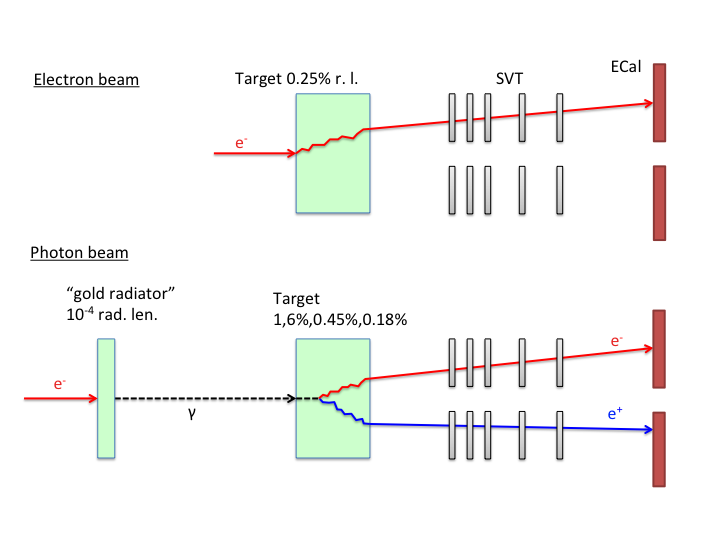
\includegraphics[ scale=0.5]{test2012/angular_measurement/pictures/photon_vs_electron_beam_schematic.png}
\caption{\small{Schematic comparison of the the setup in the test run photon beam compared to the HPS electron beam.}}\label{fig:schematic_testrun_vs_erun}
\end{figure*}
In particular, the angular distribution of the pair produced electron and positions emerging 
from the converter has comparable contributions from {\it i)} the pair production angle
and {\it ii)} the multiple Coulomb scattering of the electron and position in the converter after production, see  Fig.~\ref{fig:schematic_pair_prod}.
\begin{figure*}[]
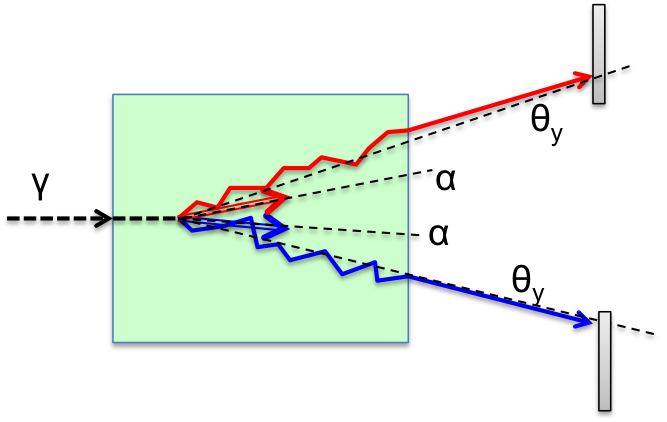
\includegraphics[ scale=0.7]{test2012/angular_measurement/pictures/pair_prod_schematics.png}
\caption{\small{Schematic description of the relevant angles for pair production in the 
test run.}}\label{fig:schematic_pair_prod}
\end{figure*}
%The contribution from the two firsboth sources to the final angular distribution are comparable. 
%FigureX 
%shows the expected distribution of the vertical angle $\theta_y$ for the $e^+e^-$ pair  coming 
%out of the converter compared to the pair production angle. {\color{red} Need this figure from Takashi.} 


%{\bf Sample Composition}\newline

The measured angular distribution in the ECal for the three converter thicknesses are shown in 
Fig.~\ref{fig:ang_distr_data} (left).  
\begin{figure*}[]
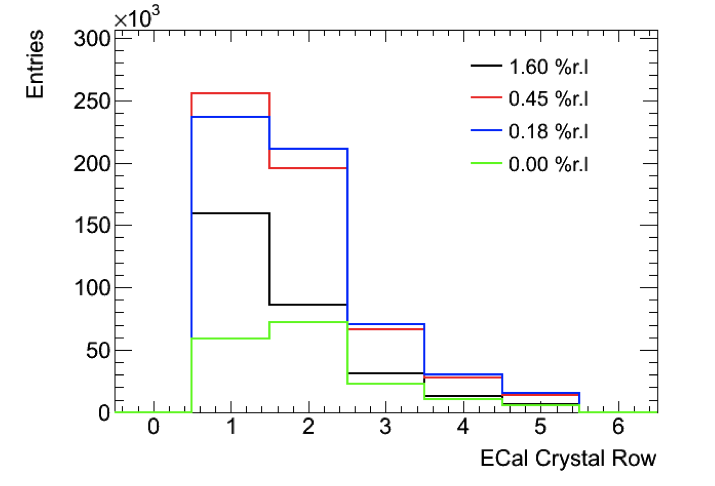
\includegraphics[ scale=0.65]{test2012/angular_measurement/pictures/rate_ecalrow_raw.png}
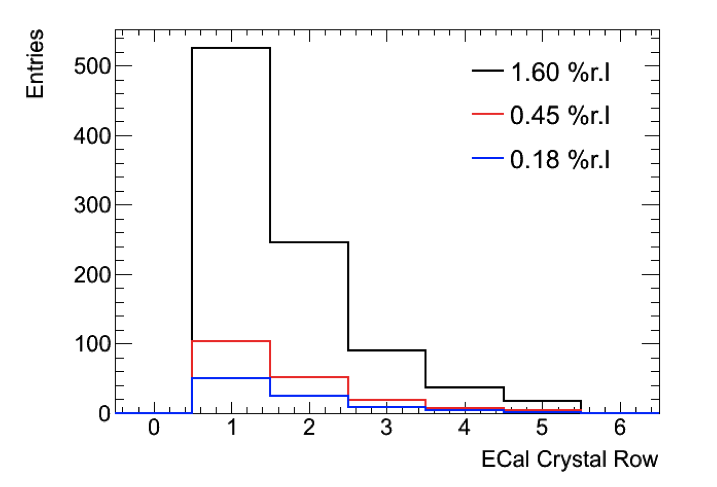
\includegraphics[ scale=0.65]{test2012/angular_measurement/pictures/rate_ecalrow_norm_subtr.png}
\caption{\small{Measured raw vertical angular distributions before (left) and after (right) 
normalization and background subtraction.}}
\label{fig:ang_distr_data}
\end{figure*}
The photon beam line during the test run produced a relatively large fraction of pairs 
originating upstream of the converter. This contribution was measured during data taking 
with "empty" converter runs i.e. removing the converter but with all other conditions 
the same. The upstream background measured in the "empty" converter runs was subtracted 
from the other runs, properly normalized using the measured integrated currents detailed in 
Tab.~\ref{tab:currents}.
\begin{table}
\centering
\begin{tabular}{|c|c|c|}
\hline
%Run & converter thickness [\%r.l.] &   start time[s]      & end time [s] & Duration [s] &       integrated beam current (nC)    \\                thickness (%r.l.)       Rate(Hz)     Recorded(Hz)  Magnet Polarity
Converter thickness & Duration &  $e^-$ on converter \\
 (\%r.l.) & (s) & (nC)    \\   
\hline
%\hline
1.6   & 911 &     24385.9     \\
%\hline
0.18   & 2640 &    193508.9  \\
%\hline
0.45  & 2149 &       140709.9  \\
%\hline
0    & 1279  &   88079.6  \\
%1349    1337323714      1337324625      51344.0926551819        54879.7343788147        1.6                     1262.120     1174.728      -1
%1351    1337324962      1337325268      24385.9185791016        26928.0426635742        1.6                     1933.479     1696.808      -1
%1353    1337325717      1337328357      193508.881838322        204325.132622242        0.18                    436.895      425.659       -1
%1354    1337328521      1337330670      140709.898532331        148839.141475141        0.45                    596.055      570.870       -1
%1358    1337331152      1337332431      88079.5567516331        92523.9428218845        0                       309.785      304.253       -1
%1359    1337332615      1337334014      91653.0026320741        91761.4541434497        0                       318.640      311.540       1
%1360    1337334136      1337336898      198670.590789914        209883.979889035        0.18                    451.067      446.510       1
%1362    1337337264      1337338713      105642.70688653         110298.553449392        1.6                     1864.090     1659.675      1
%1363    1337340178      1337340456      8556.8459701538         8556.8459701538         1.6                     1864.090     1659.675      1
\hline
\end{tabular}
\caption{{\small Measured integrated currents for the runs used to measure the angular distributions.}}
\label{tab:currents}
\end{table}
The background fraction for the there converter thicknesses was 16\%, 52\% and 71\% 
for converter thicknesses of 1.6\%, 0.45\% and 0.18\%, respectively. The background fraction was also 
cross-checked by pointing back tracks reconstructed in the SVT to identify the fraction of tracks not emanating from the converter. This can be seen in Fig.~\ref{fig:extrapol_converter} (bottom) where small 
satellite peaks at $\pm 10$~mm can be identified as tracks from the upstream background. The angular distribution, after normalization and subtracting the upstream background, are shown in 
Fig.~\ref{fig:ang_distr_data} (right).  We also checked that the contribution from photons to our triggered 
sample was less than 2\% (without angular selections which would further reduce the contribution).
%. To make sure that our distributions are dominated by $e^+e^-$ pair Since we are primarily interested in measuring the angular 
%distributions for the $e^+e^-$ pair we checked that the contribution from photons in our triggered sample are negligible. Table~\ref{tab:sample_composition} shows the sample composition. The fraction of photons that would deposit energy to reach threshold in the ECal crystals are much less than 2\% without any angular selection which will further reduce the fraction of photons. 
%\begin{table}[]
%\centering
%\begin{tabular}{c|c|c|c}
%Type & Nominal & $E>0.2$~GeV & $E>0.5$~GeV \\
%\hline
%electron & 7150 & 4938 & 3186 \\
%positron & 6019 & 4568 & 2874 \\
%$e^+e^-$ & 13169 & 9506 & 6060 \\
%photon & 2984 & 640 & 151 \\
%\hline
%\end{tabular}
%\caption{Sample composition for the photon test run.}
%\label{tab:sample_composition}
%\end{table}
%Figure~\ref{fig:extrapol_converter} (bottom) shows the vertical position of 
%reconstructed tracks in the SVT during data taking with a converter thickness of 
%1.6\% radiation length. Note the small satellite peaks visible at about $\pm 10$~mm which 
%can be identified as the upstream background when studying the same distribution from the 
%run without any converter. 
%\begin{figure*}[t]
%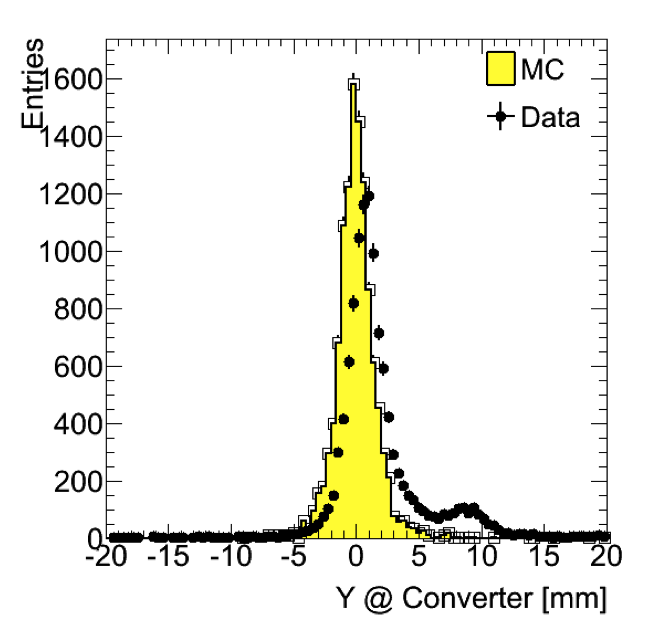
\includegraphics[ scale=0.6]{test2012/angular_measurement/pictures/tracks_at_converter_Y_top.png}
%\includegraphics[ scale=0.6]{test2012/angular_measurement/pictures/tracks_at_converter_Y_bottom.png}
%\caption{\small{Vertical position of extrapolated tracks from the SVT to the converter position.} {\color{red}Need update.}}\label{fig:tracks_at_converter}
%\end{figure*}


These measured angular distributions are compared to simulation to validate the modeling of the 
multiple Coulomb scattering. As described in more detail in Appendix \ref{app:sim}, EGS5 is used to generate 
the electromagnetic interactions in the converter while GEANT4 is used to simulate the particles after the converter.  Figure~\ref{fig:ang_distr_dataMC} shows the angular distribution comparing data and 
EGS5 normalized to 1~s of beam at 90~nA beam current. 
\begin{figure*}[t]
\includegraphics[ scale=0.25]{test2012/angular_measurement/pictures/dataMC_1351_Hit_Y_top_norm_bkgsub.png}
\includegraphics[ scale=0.25]{test2012/angular_measurement/pictures/dataMC_1354_Hit_Y_top_norm_bkgsub.png}
\includegraphics[ scale=0.25]{test2012/angular_measurement/pictures/dataMC_1353_Hit_Y_top_norm_bkgsub.png}
\caption{\small{Comparison between the observed and predicted angular 
distribution using EGS5 for converter thickness of 1.6\% (left), 0.45\% (middle) and 0.18\% 
(right).  Only statistical uncertainties are included. }}
\label{fig:ang_distr_dataMC}
\end{figure*}
The total rate measurements are in Fig.~\ref{fig:rate_vs_thickness} and summarized in 
Tab.~\ref{tab:ang_distr_dataMC}.
\begin{figure*}[t]
%\includegraphics[ scale=0.65]{test2012/angular_measurement/pictures/rate_vs_thickness_dataMC.png}
\includegraphics[ scale=0.3]{test2012/angular_measurement/pictures/dataMC_geant4.png}
\includegraphics[ scale=0.3]{test2012/angular_measurement/pictures/dataMC_egs.png}
\caption{\small{The measured rate as a function of converter thickness comparing GEANT4 (left) and EGS5 (right)}.} 
\label{fig:rate_vs_thickness}
\end{figure*}
The total systematic uncertainty was estimated to be between 10-18\% depending on the run including:  
a 5\% uncertainty on the integrated current normalization, 
alignment of the ECal, 
uncertainty from the background normalization, 
and limited Monte Carlo statistics.  
%The uncertainty from the initial gain calibration of the 
%ECal described in Sec.{\color{red} X} was estimated to be less than {\color{red} Y\%, need to check this %calibration systematic.}.
\begin{table}
\begin{tabular}{|l|c|c|c|}
\hline
Converter (\% r.l.) & 1.60 & 0.45 &	0.18 \\
\hline
EGS5 &	1162 $\pm$ 112 &	255 $\pm$ 28 &	94 $\pm$ 17	\\
\hline
GEANT4 & 2633 $\pm$ 250 & 	371 $\pm$ 38 &	114 $\pm$ 18 \\
\hline
Observed 	& 1064 $\pm$ 2 & 196 $\pm$ 1 &	92 $\pm$ 1 \\						
%Beam gap	58	13	5	132	19	6
%	EGS			G4		
%converter thickness	1.60%	0.45%	0.18%	1.60%	0.45%	0.18%
%Data [/90nC]	1064	196	92	1064	196	92
%Pred. [/90nC]	1162	255	94	2633	371	114
%Total uncertainty	112	28	17	250	38	18
%Stat	2	1	1	2	1	1
%						
%Stat MC	11	3	1	16	3	1
%Bkg norm.	14	14	14	14	14	14
%Current norm.	94	21	8	212	30	9
%Beam gap	58	13	5	132	19	6
\hline
\end{tabular}
\caption{ {\small Observed and predicted number of events for 1~s of beam at 90~nA for three different converter 
thicknesses. The uncertainty on the prediction includes systematic uncertainties. }}
\label{tab:ang_distr_dataMC}
\end{table}

In summary, the accurate modeling of the multiple Coulomb scattering is fundamental to estimate occupancies and trigger rates for HPS. EGS5 predicts the correct angular distribution across all converter thicknesses while GEANT4 overestimates the rates; with the disagreement increasing  with larger converter thickness. This preliminary result verifies our modeling of the multiple Coulomb scattering using EGS5 for HPS.
%Since EGS5 was used to generate the pair 
%angle distribution for both simulation described in the result it's interesting to see that the 
%ratio of data to the prediction varied from 0.91 (0.40), 0.77 (0.53) and 0.98 (0.81) for {\sc EGS} 
%(GEANT4) at 1.6\%, 0.45\% and 0.18\% converter thickness, respectively. If the pair angle 
%distribution were responsible for the difference between GEANT4  and EGS5 that would show up as a large shift in this ratio since the multiple Coulomb scattering contribution varies. 
%There are more work needed to go from this preliminary result to a real 
%measurement. However, this preliminary result further strengthens our confidence that 
%EGS5 is able to properly describe the large angle multiple Coulomb scattering events in the converter 
%which is important to estimate our occupancy and trigger rates for HPS (see Sec.~\ref{sec:performance}).






